% \newgeometry{left=2cm}
\chapter{外文资料原文}
\label{cha:engorg}

\title{Multimodal Deep Learning for Robust RGB-D Object Recognition}
\begin{center}
{\footnotesize Andreas Eitel, Jost Tobias Springenberg, Luciano Spinello, Martin Riedmiller, Wolfram Burgard}
\end{center}

\begin{figure}[ht]
   \centering
     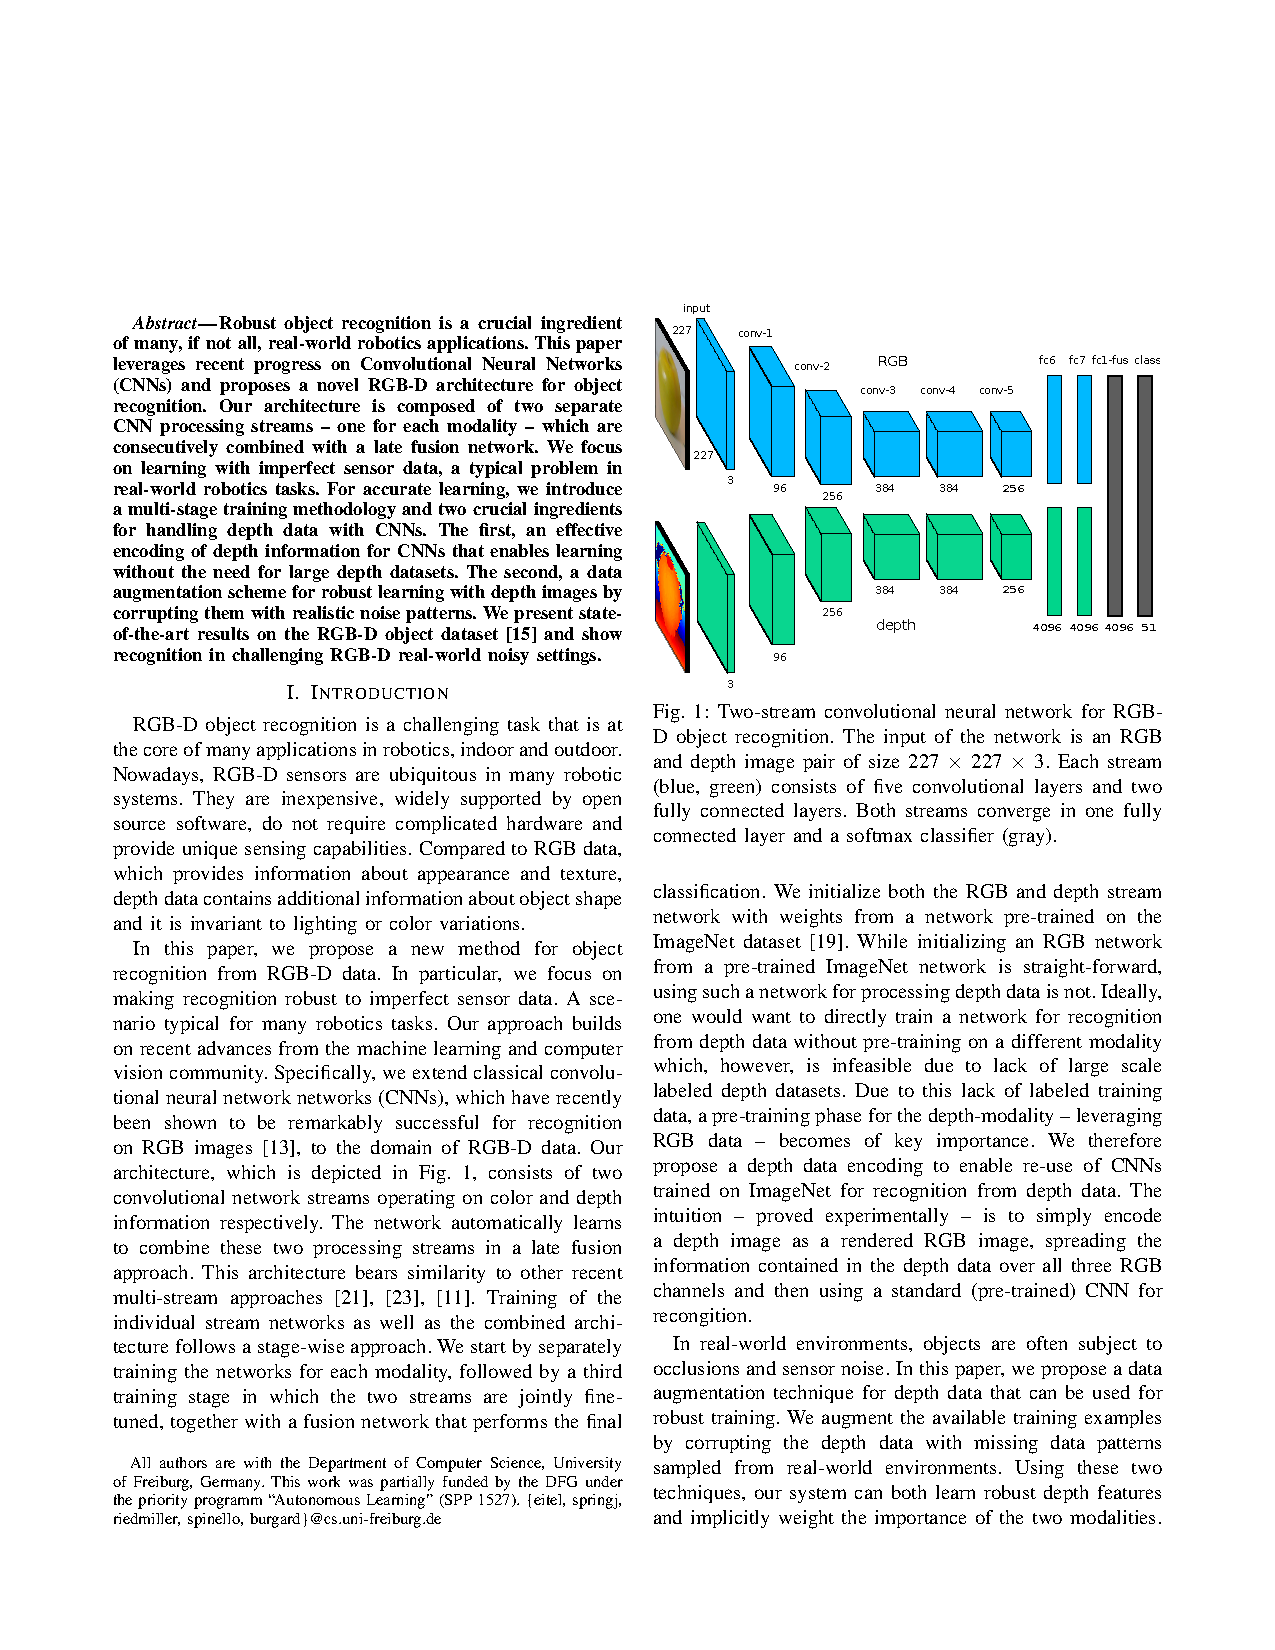
\includegraphics[page=1,width=0.95\textwidth]{MultimodalRGBD}
\end{figure}

% \restoregeometry

\begin{figure}[ht]
   \centering
     \includegraphics[page=2,width=0.95\textwidth]{MultimodalRGBD}
\end{figure}

\begin{figure}[ht]
   \centering
     \includegraphics[page=3,width=0.95\textwidth]{MultimodalRGBD}
\end{figure}

\begin{figure}[ht]
   \centering
     \includegraphics[page=4,width=0.95\textwidth]{MultimodalRGBD}
\end{figure}

\begin{figure}[ht]
   \centering
     \includegraphics[page=5,width=0.95\textwidth]{MultimodalRGBD}
\end{figure}

\begin{figure}[ht]
   \centering
     \includegraphics[page=6,width=0.95\textwidth]{MultimodalRGBD}
\end{figure}

\begin{figure}[ht]
   \centering
     \includegraphics[page=7,width=0.95\textwidth]{MultimodalRGBD}
\end{figure}

\chapter{外文资料的调研阅读报告或书面翻译}

\title{\heiti 多模态深度学习与稳定的RGB-D物体识别}

{\heiti 摘要:}
稳定的物体识别是许多现实世界中机器人应用问题中的关键因素。本文基于卷积神经网络(CNN)的最新进展,提出了一种新型的RGB-D物体识别架构。我们的体系结构是由两个独立的CNN处理流组成的——每个模态对应一个处理流——并继续与后期的融合网络相结合。我们关注不完美的但是在现实世界经常遇到的有噪音的传感器数据。为了获得准确的学习,我们引入了一个分级的训练方法和两个适用于CNN的用来处理深度数据的技巧。第一个技巧是,使用一种对CNN有效的深度信息编码,使学习不需要很大的深度数据集。第二个技巧是,使用一种适用于深度信息的数据增强方法,用现实的噪音模式破坏它们。我们提出的识别架构在RGB-D物体数据集[15]上获得了最先进的识别成果,并且在富有挑战性的现实世界RGB-D数据中也获得了较好的识别结果。

\section{引言}

RGB-D物体识别是一项具有挑战性的任务。它在机器人领域以及室内和室外的许多应用中都是核心技术。如今,RGB-D传感器无处不在。许多机器人系统都可以使用价格便宜,广受支持的开源软件,而不需要使用复杂的硬件来提供独特的感知能力。RGB数据,提供了有关外观和纹理的信息;而深度数据则包含有关物体形状的附加信息,它是不随亮度或颜色而改变的,所以对物体识别具有特殊的意义。

在本文中,我们提出了使用RGB-D数据的新的对象识别方法。特别是,我们关注在有噪声的情况下——一个典型的机器人任务的背景下——稳健地识别不完善的传感器数据。我们的方法建立在机器学习和计算机视觉的最新研究成果上。具体地说,我们扩展了经典的卷积神经网络(CNN),CNN最近被证明在RGB图像[13],以及RGB-D数据识别方面获得了显着的成功。我们的工作的结构如图 1所示。由两个关于颜色和深度操作卷积网络流分别处理两种信息。由网络自动学习这两种处理流在后期的融合策略。这种架构与其他最近的多流的方法[21],[23],[11]相比有着比较大的相似度。将训练出来的单个网络流以及将合并的部分使用分阶段训练的方式是很有效果的。我们启动训练网络分别对于每个模态,以及两个模态融合的阶段训练微调,与执行网络连接,最终的融合网络会做出最总的分类结果预测。我们初始化RGB和深度流网络所用的权值是从一个在ImageNet数据集[19]上预先训练好的神经网络模型继承来的。尽管我们可以直接使用这个在颜色信息中训练好的模型来分类RGB信息,但是并不能直接使用它来分类深度信息。理想情况下,我们可以直接使用深度数据训练出一个适合的CNN模型,而不用使用其它模态的数据。然而,实际中是不可行的,因为缺乏大量已经标记的深度数据集。由于缺乏标记的训练的数据,深度模态在训练的初始状态需要借鉴使用RGB数据训练出的模型,这是至关重要的。因此,我们提出了一种深度数据编码,以便再利用在ImageNet中训练好的CNN来识别深度数据。这个已经被试验验证的直觉是简单地将深度图像编码作为RGB图像,在三个RGB信道中都填上深度数据的信息,然后使用标准(预训练的)CNN做识别。

在现实环境中,对象是经常受到遮挡和传感器噪声的影响。在本文中,我们提出了一种深度数据增强技术,该技术可用于有噪声场景的稳定的训练。我们增加了训练样例,通过使用从现实环境采样的缺失数据型态来破坏深度数据。使用这两种技术,我们的系统既可以学习稳定的的深度识别和隐式加权两种模式的重要性。
 
我们测试了我们的方法来验证我的想法:我们在RGB-D的数据集中使用我们的方法做分类以测试我们方法的精度,然后在有现实世界噪音的数据集中测试我们方法的稳健性。对于第一个,我们的实验结果表明,我们的工作性能优于所有现有技术在Lai等人的RGB-D对象数据集[15]中的分类结果。第二,我们表明我们的数据增强方法提高了在充满挑战的现实世界和有噪声条件下的RGB-D场景的数据集[16]中的识别准确率。

\section{相关工作}

我们的做事涉及到两块重要的工作,分别是卷积神经网络(CNN)用来做物体识别,和应用计算机视觉的方法去解决使用RGB-D数据做识别中遇到的问题。尽管本文不会做一个包含CNN和物体识别的综合广泛的文献综述,我们还是会快速的点明我们的方法和近期已有的工作有什么区别。

在众多成功的RGB-D物体识别算法中,有很大一部分都是使用手工设计的信息,比如SIFT与深度信道的多种形状特征结合 [15],[16]。然而,随着它们在许多计算机视觉的问题中都获得了成功,非监督学习的特征学习方法也在最近被拓展到了RGB-D识别的领域。Blum等人[3]提出了一种基于K-Means的RGB-D描述符。更加近期的工作包括Bo等人[5]提出的分层匹配追踪,一种分层级的稀疏编码方法,可以从多个输入信道学习特征。Socher等人[22]提出了一种不同的方法,这种方法依靠将卷积过滤器和递归神经网络(一种特殊的再现神经网络)结合起来作为识别层级。Asif等人[1]报告了一种可以使用随机森林瀑布来提高识别准确率的分类器,这种分类器也是分层融合的。最后,在最近Schwarz等人的独立工作中[20],提出了使用ImageNet上预先训练出的CNN提取出的RGB-D特征来做RGB-D识别。尽管他们也使用有两个网络流组成的分类架构,他们并没有对CNN使用RGB-D做微调,而只是使用原有的神经网络。有趣的是,他们还发现了简单的上色方法可以使深度信息获得较好的识别效果,甚至可以与许多复杂的预处理的效果相当。与他们的工作不同,我们获得了更高的准确率,并且训练出一个端对端的融合CNN:输入未加工的像素信息,直接输出分类信息,整个过程是一个监督学习的过程,并且使用了在相关任务中训练的模型。所以,我们的CNN学习到的特征从结构上与现有的其他任务中的特征是可区分的。使用CNN做物体识别在计算机视觉和机器学习领域有着很长的历史。尽管人们都知道CNN在监督的图像识别、分类任务中(比如MNIST [17])很早就可以获得较高的准确率,最近CNN方法已经不仅仅可以在例如大规模图例如分类任务[13]、物体识别[9]、语义分割[8]等方面中超过经典的方法,还可以产生在多种任务中转换的特征[7],[2]。计算能力强大的高性能计算系统使得这个最近的成功的故事成为可能,而大规模图像数据集的出现也起了不可或缺的作用,比如ImageNet[19]。




虽然大多数的深度学习工作的重点是二维图像,最近的研究也已经包含使用深度信息用于改进场景分类和物体检测[6],[10]。其中,和我们最相似的是Gupta等人[10]提出的比较普适的使用R-CNN检测器适用于深度信息的方法[9]。详细地说,他们使用已经在RGB图片数据集上训练好的大型CNN去提取深度信息中的特征,将深度信息编码到三个信道(使用HHA编码)。更加具体地说,他们对每一个像素点,编码了离地面的高度,水平的距离和像素层面上的表面法向和重力之间的角度。我们的融合网络架构与他们的使用预先训练的神经网络有着相似之处。不过我们的方法与他们的方法的不同之处在于,将深度信息编码为颜色信息的过程和融合两种模态的融合方法。对于编码过程,我们提出了一种对于深度图片的编码方法,我们的这种方法不依赖于复杂的预处理,但是与HHA相比获得了性能上的改进。为了实现模态融合,我们在原有神经网络的基础上有加了一层融合层,使得我们的识别架构可以自动的学习出对于识别的融合的策略,这和仅仅在提取出的信息的上面训练出一个线性分类器先比有着更好的表现。多刘的架构已经被人用于多种任务,包括识别[21],检测[11],图片提取[23]。一个最近的有关深度和图片信息融合的不同网络结构在Saxena等人的研究中给出[18]。在哪里,作者比较了不同的多模态学习的模型:
\begin{enumerate}
\item 早期融合,其中输入图像被级联到现有的图像RGB通道并一起处理;
\item 我们定义为后期的融合,其中的功能是为每个单独训练的情态,然后在更高层融合;
\item 将早期和晚期的方法结合;
\end{enumerate}
得出的结论是后期融合(2)和早期和后期相结合的办法最适合把握问题的关键特征,有利于检测。相比与他们的工作,我们的模型是使用类似于后期融合的方法,但又有着很大的不同。[18]使用逐层无人监督的训练方法,他们的规模(包括其网络和输入图像数据集的大小
)都比我们要小一个数量级。

\section{用于RGB-D物体识别的多模态架构}

该架构的概述在图 1中给出。 我们的网络由两个流(在图 1中的顶部蓝色和底部绿色)——分别处理RGB和深度数据——然后在更晚的阶段被融合在一起的方法。每个流由一个已经在ImageNet数据集中训练好的深度CNN组成(我们使用Krizhevsky等人[13]训练的CaffeNet[12]作为预训练模型)。使用预先训练的神经网络的关键原因是我们希望在优先的数据量上使用一个包含着百万级别的参数的大型CNN。(例如,见Yosinski等人 [25]在最近对于此的讨论)我们首先对两个模态的信息进行预处理,然后使用分阶段的方法训练我们的多模态CNN网络。我们首先对每个模态的CNN进行微调,然后使用两个模态微调出的模型,将它们结合在一起,联合的训练出融合网络的参数。不同的步骤将会在一下小节被详细说明。

\subsection{输入预处理}

要充分利用在ImageNet上预先训练的CNN的力量,我们预处理RGB和深度模态的输入数据,使得它与原ImageNet的输入兼容。具体地说,我们使用在CaffeNet[12]中的参考实现,这个模型接受227 $\times$ 227像素的RGB作为输出。这227 $\times$ 227个像素点通常是用256 $\times$ 256个像素点的RGB图片缩放而成的。处理的第一步要缩放图片到合适的大小。而缩放最简单的方法就是使用图片翘曲,放弃原始图片的长宽比例直接缩放。这在图片3(中)中有所阐释。我们发现在我们的试验中,这个处理过程会降低识别的准确率——我们把这个问题归因于目标物体形状信息的损失(见IV-C)。所以我们设计了一种不同的预处理方法:将长边缩放到256个像素,得到一个256 $\times$ N或者 N $\times$ 256的图片。然后我们将缩放后的图片沿短边像瓷片一样平铺到256 $\times$ 256的空间上。得到的最终的颜色图片和深度图片在物体边界处展示出一种人造的环境(见图 3)。我们对颜色信息和深度信息都是用这种方法进行预处理。

对于RGB图像,在预处理缩放之后可直接使用作为CNN的输入,而缩放之后的深度数据需要额外的步骤。为了实现这一点,我们可以回想一下是用ImageNet训练的神经网络已经被训练去识别某个特别的图像输入分布(即天然相机图像),它与深度传感器得到的标志物体距传感器的距离的信息是不相容的。尽管如此,通过查看一个典型的家用物品的深度图片(参考图 4),可以得出结论,许多定性
出现在RGB图像中的特征,比如边、角、阴影区域等模式,也会出现在深度图片中。这种认识引出了这种想法:简单地使用深度数据渲染出的三通道的RGB图片作为用于在ImageNet [10]上训练的CNN的输入。我们将比较这些深度图片渲染的方法与我们的做法的不同之处。两种最流行的深度图片编码是:
\begin{enumerate}
\item 深度数据渲染成灰度值,并复制灰度值到所要求的三个通道作为神经网络输入;
\item 利用表面法线,其中每个法线矢量的维度对应于一个信道所产生的图像。
\item 一个更复杂的方法,称为HHA编码[10],对每一个像素点的三个信道,编码了离地面的高度,水平的距离和像素层面上的表面法向和重力之间的角度。
\end{enumerate}


我们提出第四种有效并且计算成本较低的,将信息编码为彩色图像的方法,我们发现此种方法在物体识别中的表现要比HHA编码更好。我们的方法首先要标准化所有的深度值到0和255。然后,我们应用一个喷射颜色表将深度信息从单通道输入转换到一个三通道图像(给深度着色)。对于尺寸为 W $\times$ D 的深度图像中的每个像素(i,j)中,我们将距离信息映射为颜色值,从红色(附近)到绿色再到蓝色(远),并将这些信息分散到三个信道。这三个信道的边缘往往对应着有用的对象边界。因为我们使用的卷积神经网络是用RGB图像训练的,着色过程提供了深度信息和RGB图像之间足够多的共同结构,所以可以使用CNN来处理深度信息(对不同深度预处理方法之间的比较参照图 2)。

\section{实验}

我们在华盛顿大学的RGB-D物体数据集[15]上评估对我们的多模态神经网络体系结构。这个数据集包括属于51个不同类别的日常家用物品。作为额外实验,我们使用了RGB-D场景数据集中的被部分遮挡的物体来评估的算法的可靠性以及对于现实世界数据的分类能力。

\subsection{实验设置}

所有实验都是使用开源的Caffe框架[12]。如先前所描述,我们使用
的CaffeNet作为我们融合网络的基础。它由五个卷积层(在第一、第二和第五之后需要最大池化),其次是两个完全连接层和SOFTMAX分类层。除了最后一层之外所有的层都用到了修正线性单元。我们使用预先训练的模型的前八层的权重和偏差来初始化我们网络的前八层,丢掉了最后的SOFTMAX分类层。然后我们继续使用分阶段训练。第一阶段(分别训练RGB和深度信息)当中所有信息层的参数都按照一种固定学习率(learning rate)的模式在改变(最开始学习率取为0.01,经过20K次迭代后变为0.001,并在30K次迭代后停止训练)。在第二阶段(训练融合网络,20K次迭代,使用大小为50的mini-batch),我们尝试微调了所有的权值,但是最后发现将上一阶段训练出的两个模态的各自的CNN网络权值固定(设定它们的学习率为0),只微调融合部分的网络效果更好。我们从此任务的十种数据分割方法中随机选出一种分割作为确认分割,而训练的迭代次数是基于在确认分割上的测试结果所选定的。如果没有特殊说明,我们使用固定为0.9的momentum和固定为128的mini-batch。我们还使用了常见的数据增强的做法:在较大的256 $\times$ 256的图片中随机选取大小为227 $\times$ 227子图像,然后实行随机水平翻转。我们使用一块NVIDIA 780显卡,训练单支神经网络流需要10个小时。

\subsection{RGB-D物体数据集}

华盛顿RGB-D数据集的物体由41877个含家用物品RGB-D图像组织成,它们分别属于51个不同的种类的一共300个实例。这些图像是在三个不同视点捕捉的。我们使用间隔5帧的采样来评估我们的算法。我们使用和Lai等
人 [15]相同的十折交叉验证分割,来评估我们的方法在具有挑战性的类别识别任务中的表现。每个分割包括大约35000组训练图像和7000组测试图像。每一个对象类中,一个是被留下做测试的。所以我们在剩下的300-51 = 249个实例中进行训练。在测试时CNN的任务是给每个之前没见过的实例分类。

表I显示了我们的多模态CNN识别的平均准确率与以往工作中的最好结果的对比。
我们得到的最佳结果,使用喷射着色(FUS-CNN JET)与RGB和深度信息时(84.1 $\pm$ 2.7\%和83.8 $\pm$ 2.7\%时,当分别使用RGB或深度模式时),得到的91.3 $\pm$ 1.4\%的整体准确率,比就我们所知的所有前人的工作都要高。
我们还展示了使用需要更多计算的HHA编码的结果(FUS-CNN HHA)。从表中可以看出,HHA编码并没有带来表现的提升。我们提出的着色方案要比HHA的表现(FUS-CNN HHA)稍好一点,同时需要更少的计算资源。整体来说我们的试验结果表明,一个预先训练的CNN可以用来识别深度数据,只需要预先使用我们的着色方法对深度信息进行预处理即可。除了表中展示的结果,我们还做了有关不不同的融合网络结构的试验。具体来说,如果将融合中间层(fc1-fus)去掉,识别准确率会稍微下降至91\%。增加融合层也不能得到更好的结果。最终,图6展示了每个类的召回率(recall),其中大约一半物体实现了约等于99\%的召回率。

\subsection{深度域适应RGB-D场景}

为了测试我们的深度信息增强方法在真实世界中的效果,我们进行了在更具挑战性的RGB-D场景数据集中的附加实验。此数据集包括六个对象类(与RGB-D物体数据集重叠)和大量受噪声影响的深度图像。在这个实验中,我们训练的两个单流深度神经网络,使用物体数据训练,并使用场景数据集进行测试。
此外,我们假设一定正确的边框已经被给出,这种就可以只测试识别的性能。第一个“基准”神经网络由第III-B.1中描述的方法所训练出来,标签的总数目M = 6。第二神经网络是使用III-C中提出的深度信息增强方法训练出来。
该实验的结果展示于表II(中间和右栏),报告了每个对象类在所有八个视频序列中的识别精度。
从该表中可以看出,经过适应的网络是明显的(右边使用数据增强方法训练的列)优于基准模型中的所有类,这显然表明额外的领域适应性对于在现实世界中的场景的稳健识别是有必要的。
然而,一些类(例如,盖,碗,苏打罐)从噪音训练中获得提升比其他类更高(例如,手电筒和咖啡杯)。图 4中描绘的厨房场景给出了一些有关此结果的视觉直觉。
另一方面,一些对象(例如,汽水罐)往往会出现非常嘈杂对象边界和表面,因此它们使用适应方法会显示出较大的识别性能改进。
另一方面,小物体(例如,手电筒),这些物体经常是在桌子上拍的,要么不受噪音影响或只受轻微的影响,因此这些噪音容易被我们的数据增强方法完全擦除。图 7显示了几个被基准网络错误分类,但是可以使用我们的数据增强方法正确分类的例子。
我们还测试了如图 3所描述的不同的图像缩放技术的效果。如表II所示,标准图像变形表现的不是很好,这支持了我们的直觉,即形状信息会在预处理过程中丢失。

\subsection{深度编码方法的比较}

最后,我们进行了实验,以比较图 2所描述的不同的深度编码及方法。对于图像的缩放,我们使用了图 3描述的需处理方法,并使用不同的深度信息编码方法进行了测试。
我们考虑到两种场景:
\begin{enumerate}
\item 使用单通道深度图像做训练
\item 对每一种编码方法,只使用第三节-B.1的方法来预处理深度信息,然后作为训练集。
\end{enumerate}
当从头训练时,初始学习率设定为0.01,然后在40K次迭代后改变到0.001。经过反复迭代60K次后停止。训练更多的迭代次数并不能进一步提高精度。通过查看表III中的结果,很显然训练从头训练的表现不如使用已有模型微调的效果好。在后一种情景下,结果显示最简单的编码方式(将深度信息转换为灰度图片)的识别效果要显著差于其他的方法。在其他的编码方法中(所有这些方法都会给深度信息着色),平面法向和HHA编码需要额外的图片图像预处理,而使用我们提出的深度-喷射着色的方法几乎不需要任何计算资源。一个HHA编码在此情景下表现的不尽人意的可能原因是此数据库中的图片都是放在一个可以旋转的托盘中,他们的高度都是相同的。所以HHA中用到的高度信道就无法包含用于分类的其他信息。在本实验中,使用平面法线要比深度-jet编码的表现稍好一点。所以我们使用平面法线的编码来试验了我们的融合网络,不过这并没有进一步提高识别表现。具体地说,测试集上的识别准确率是91.1 $\times$ 1.6,这与我们在表I中报告的结果相差不大。

\section{结论}

我们提出了一种可以用于RGB-D物体识别,并且在RGB-D物体数据集[15]中实现了当前最好表现的新型多模态神经网络结构。我们的方法是由二个卷积神经网络流组成,这两个CNN流在分类前可以从RGB和深度信息中自动地提取和融合信息。我们利用一种有效的编码方式,把深度数据编码为图像,使我们能够充分利用在ImageNet数据集中训练的大型神经网络进行对象识别。我们提出了一种新的深度数据增强方法,旨在提高对嘈杂的现实世界深度数据的识别准确率,以便适用于典型的机器人场景。目前大量的实验结果证明了我们方法的正确性,以及它能够从两个模态学习丰富的特征。我们的方法还可以在现实世界环境中稳定地识别物体,并证明了噪声感知训练是有效的,并且可以被用来改进RGB-D场景数据集[16]的识别精度。